\begin{enumerate}
	\item 		Obtain the Minimal Form for the Boolean Expression
\label{prob:2013/d/6/d}
\hfill (CBSE 2013)
		\begin{align}
\label{eq:2013/d/6/d}
H(P,Q,R,S)=\sum(0,1,2,3,5,7,8,9,10,14,15)
		\end{align}
	\item Write the POS form for the function G shown in Table
\ref{tab:2013/c/6/d}.
\label{prob:2013/c/6/d}
\hfill (CBSE 2013)

		\begin{table}[!ht]
			\centering
		\begin{tabular}{ |c |c |c |c |}
 \hline
 U  &  V  &  W  &  G\\
 \hline
 0  &  0  &  0  &  1\\
 \hline
 0  &  0  &  1  &  0\\
 \hline
 0  &  1  &  0  &  1\\
 \hline
 0  &  1  &  1  &  0\\
 \hline
 1  &  0  &  0  &  1\\
 \hline
 1  &  0  &  1  &  0\\
 \hline
 1  &  1  &  0  &  0\\
 \hline
 1  &  1  &  1  &  1\\
 \hline
 \end{tabular}
			\caption{}
\label{tab:2013/c/6/d}
 \end{table}
	\item Reduce the following Boolean Expression to its simplest form using K-Map 
\label{prob:2015-1/c/6/d}
\hfill (CBSE 2015)
		\begin{align}
\label{eq:2015-1/c/6/d}
			F(X,Y,Z,W)=(0,1,4,5,6,7,8,9,11,15)
		\end{align}
	\item 
		Derive a Canonical POS expression for a Boolean function F, represented by the following truth table 
\label{prob:2015-1/c/6/c}
\hfill (CBSE 2015)
		\begin{table}[!ht]
			\centering
		\begin{tabular}{|c|c|c|c|}
	\hline
X & Y & Z & F \\
\hline
0 & 0 & 0 & 1 \\  
\hline
0 & 0 & 1 & 0 \\ 
\hline
0 & 1 & 0 & 0 \\
\hline
0 & 1 & 1 & 1 \\
\hline
1 & 0 & 0 & 1 \\  
\hline
1 & 0 & 1 & 0 \\ 
\hline
1 & 1 & 0 & 0 \\
\hline
1 & 1 & 1 & 1 \\
\hline
\end{tabular}
		\caption{}
\label{tab:2015-1/c/6/c}
\end{table}
	\item 
\label{prob:2015/c/6/d}
\hfill (CBSE 2015)
		Reduce the following Boolean Expression to its simplest form using K-map
		\begin{align}
\label{eq:2015/c/6/d}
F(X,Y,Z,W)= \sum (0,1,6,8,9,10,11,12,15)
		\end{align}
	\item Reduce the following Boolean Expression to its simplest form using K-map.
\label{prob:2016/c/6/d}
\hfill (CBSE 2016)
		\begin{align}
\label{eq:2016/c/6/d}
			F(X,Y,Z,W)= \sum(2,6,7,8,9,10,11,13,14,15)
		\end{align}
	\item Derive a Canonical POS expression for a Boolean function  F, represented in Table
\ref{tab:2016/c/6/c}
\hfill (CBSE 2016)
\label{prob:2016/c/6/c}
		\begin{table}[!ht]
			\centering
			\begin{tabular}{|c|c|c|c|}
	\iffalse
	{0.8\textwidth} { 
  | >{\centering\arraybackslash}X 
  | >{\centering\arraybackslash}X 
  | >{\centering\arraybackslash}X | 
  | >{\centering\arraybackslash}X |
  }
  \fi
 \hline
 P & Q & R & F(P,  Q,  R) \\
 \hline
 0  & 0  & 0 & 0  \\
\hline
0  & 0  & 1 & 1  \\
\hline
0  & 1  & 0 & 1  \\
\hline
0  & 1  & 1 & 0  \\
\hline
1  & 0  & 0 & 0  \\
\hline
1  & 0  & 1 & 0  \\
\hline
1  & 1  & 0 & 1  \\
\hline
1  & 1  & 1 & 1  \\
\hline
\end{tabular}
			\caption{}
\label{tab:2016/c/6/c}
		\end{table}
	\item Verify the following 
\hfill (CBSE 2016)
\label{prob:2016/c/6/a}
		\begin{align}
\label{eq:2016/c/6/a}
A'+B'C = A'B'C' + A'BC' + A'BC + A'B'C + AB'C
		\end{align}


	\item Reduce the following boolean expression to it's simplest form using K-Map
\hfill (CBSE 2017)
\label{prob:2017-1/c/6/d}
		\begin{align}
F(X,Y,Z,W) = \sum(0,1,2,3,4,5,10,11,14)
\label{eq:2017-1/c/6/d}
		\end{align}
	\item
		Reduce the following Boolean Expression to its simplest form using K-Map.
\hfill (CBSE 2017)
\label{prob:2017/c/6/d}
		\begin{align}
E(U,V,Z,W)=   (2 , 3 , 6 , 8 , 9 , 10 , 11 , 12 , 13 )
\label{eq:2017/c/6/d}
		\end{align}
	\item Derive a canonical POS expression for a Boolean function $G$, represented by Table 
\ref{tab:2017/c/6/c}
\label{prob:2017/c/6/c}
\hfill (CBSE 2017)
		\begin{table}[htbp]
 \begin{center}
    \begin{tabular}{|l|c|c|c|c|c|c|c|c|} \hline 
  \textbf{X}& \textbf{Y} & \textbf{Z} &\textbf{G(X,Y,Z)} \\
 \hline
 0&0&0&0\\ \hline
0&0&1&0 \\ \hline
0&1&0&1\\ \hline
0&1&1&0  \\ \hline
1&0&0&1\\ \hline
1&0&1&1\\ \hline
1&1&0&0\\ \hline
1&1&1&1\\ \hline
\end{tabular}   
\end{center}
\caption{}
\label{tab:2017/c/6/c}
\end{table}
\item Derive a canonical POS expression for a Boolean function $FN$, represented by Table 
\ref{tab:2018/c/6/c}.
\label{prob:2018/c/6/c}
\hfill (CBSE 2018)
		\begin{table}[!ht]
			\centering
\begin{tabular}{|l|c|r|l|c|}
    \hline % <-- Alignments: 1st column left, 2nd middle and 3rd right, with vertical lines in between
      \textbf{X} & \textbf{Y} & \textbf{Z} & \textbf{FN(X,Y,Z)}\\
      \hline
      0 & 0 & 0 & 1\\
\hline
      0 & 0 & 1 & 1\\
\hline
      0 & 1 & 0 & 0\\
\hline
      0 & 1 & 1 & 0\\
\hline
      1 & 0 & 0 & 1\\
\hline
      1 & 0 & 1 & 0\\
\hline
      1 & 1 & 0 & 0\\
\hline
      1 & 1 & 1 & 1\\
      \hline      
   \end{tabular}
\caption{}
\label{tab:2018/c/6/c}
   \end{table}

\item 
	Reduce the following Boolean expression in the simplest form using K-Map.
		\begin{align}
F(P,Q,R,S) = \sum (0,1,2,3,5,6,7,10,14,15)
		\end{align}
\hfill (CBSE 2019)
\label{prob:2019/c/6/d}
%
\item Fig. \ref{fig:2020/gate/ec/10} below shows a muliplexer where S0 and S1 are the select lines, I0 to I3 are the input lines, EN is the enable line and F(P,Q,R) is the output. Find the boolean expression for output F as function of inputs P,Q,R using K-map. 
%
\label{prob:2020/gate/ec/10}
\hfill (GATE EC 2020)
\begin{figure}[ht]
\centering
	\includegraphics[width=1\columnwidth]{figs/2020-gate-ec-10.png}
\caption{}
\label{fig:2020/gate/ec/10}
\end{figure}
%
\item
	The four variable function $f$ is given in terms of min-terms as
		\begin{align}
	    f(A,B,C,D) = \sum m(2,3,8,10,11,12,14,15)
\label{eq:1991/gate/ec/9}
		\end{align}
	    Using the K-map minimize the function in the sum of products form. 
\label{prob:1991/gate/ec/9}
\hfill (GATE EC 1991)
\item Find the logic realized by the circuit in Fig. 
\ref{fig:1992/gate/ec/1/22}.
\label{prob:1992/gate/ec/1/22}
\hfill (GATE EC 1992)
\begin{figure}[ht]
\centering
	\includegraphics[width=1\columnwidth]{figs/1992-gate-ec-1-22.png}
\caption{}
\label{fig:1992/gate/ec/1/22}
\end{figure}
\item
	A combinational circuit has three inputs A, B and C and an output F. F is true only for the following input combinations. 
\hfill (GATE EC 1992)
\label{prob:1992/gate/ec/2/9}
	\begin{enumerate}
		\item A is false and B is true 
		\item A is false and C is true 
		\item A, B and C are all false 
		\item A, B and C are all true 
	\end{enumerate}
	\begin{enumerate}
\item Write the truth table for F. use the convention, true = 1 and false = 0. 
\item Write the simplified expression for F as a Sum of Products. 
\item Write the simplified expression for F as a product of Sums.
\end{enumerate}
\item Draw the logic circuit for Table 
\ref{tab:1993/gate/ec/5/7} using only NOR gates.
\label{prob:1993/gate/ec/5/7}
\hfill (GATE EC 1993)
	\begin{table}[!ht]
		\centering
		\begin{tabular}{|c|c|c|c|}
\hline
\textbf{C} &\textbf{B} & \textbf{A} & \textbf{Y} \\
\hline
0 & 0 & 0 & 1 \\  
\hline
0 & 0 & 1 & 1 \\ 
\hline
0 & 1 & 0 & 1 \\
\hline
0 & 1 & 1 & 0 \\
\hline
1 & 0 & 0 & 1 \\  
\hline
1 & 0 & 1 & 0 \\ 
\hline
1 & 1 & 0 & 0 \\
\hline
1 & 1 & 1& 0\\
\hline
\end{tabular}
\caption{}
\label{tab:1993/gate/ec/5/7}
\end{table}
\item
	Implement the following Boolean function in a 8x1 multiplexer.
\label{prob:1993/gate/ec/14}
\hfill (GATE EC 1993)
		\begin{align}
\label{eq:1993/gate/ec/14}
 Q = BC + ABD' + A'C'D  
		\end{align}
	\item Minimize the following Boolean function in 
\ref{eq:1999/gate/ec/2/10}.
\label{prob:1999/gate/ec/2/10}
		\begin{equation}
\label{eq:1999/gate/ec/2/10}
F= A'B'C'+A'BC'+A'BC+ABC'
\end{equation}
%
\item Find the Boolean expression for Table
\ref{tab:2005-gate-ec-54}.
\label{prob:2005-gate-ec-54}
\hfill (GATE EC 2005)
	\begin{table}[htbp]
		\centering
    \begin{tabular}{|l|c|c|c|c|c|c|c|c} \hline \textbf{A}
  & \textbf{B} & \textbf{C} & \textbf{X} \\
 \hline
        0&0&0&0 \\
        \hline
        0&0&1&0 \\
        \hline
        0&1&0&0 \\
        \hline
        0&1&1&1 \\
        \hline
        1&0&0&0 \\
        \hline
        1&0&1&0 \\
        \hline
        1&1&0&1 \\
        \hline
        1&1&1&0  \\
        \hline
\end{tabular}   
\caption{}
\label{tab:2005-gate-ec-54}
\end{table}
\item Minimize the logic function represented by the following Karnaugh map.
\label{prob:2010-gate-ee-52}
\hfill (CBSE 2021)
	\begin{karnaugh-map}[4][2][1][$YZ$][$X$]
		\manualterms{1,1,0,1,0,0,0,1}
	%	\implicant{0}{1}
	%	\implicant{3}{7}
	\end{karnaugh-map}	
\item Find the output for the Karnaugh map shown below
\label{tab:2019-gate-ec-34}
\hfill (GATE EE 2019)
	\begin{karnaugh-map}[4][4][1][$PQ$][$RS$]

		\minterms{1,3,4,5,7,6,12,13,15,14}
		\maxterms{0,2,8,9,10,11}

%		\implicant{4}{14}
%		\implicant{1}{7}
	\end{karnaugh-map}
\item The propogation delays of the XOR gate, AND gate and multiplexer (MUX) in the circuit shown in the Fig.
\ref{fig:2021-gate-ec-31}
	are 4 ns, 2 ns and 1 ns, respectively.
\label{prob:2021-gate-ec-31}
If all the inputs P, Q, R, S and T are applied simultaneously and held constant, the maximum propogation delay of the circuit is
\hfill (Gate EC-2021)
\begin{enumerate}
	\item 3 ns \item 5 ns \item 6 ns \item 7 ns
\end{enumerate}
\begin{figure}[!htb]
	\centering
\input{gate/2021/31/figs/diagram.tex}
	\caption{}
\label{fig:2021-gate-ec-31}
\end{figure}
\item 
\label{prob:2012-gate-ec-19}
Consider the 2-bit multiplexer(MUX) shown in the figure. For output to be the XOR of R and S, the values for $ W,X,Y$ and $Z$ are ? 
\hfill (GATE EC-2022)
\begin{figure}[h]
\input{gate/2022/19/figs/fig1.tex}
\caption{}
\label{fig:2012-gate-ec-19}
\end{figure}
\begin{enumerate}
\item $W = 0, X = 0, Y = 1, Z = 1$
\item $W = 1, X = 0, Y = 1, Z = 0$
\item $W = 0, X = 1, Y = 1, Z = 0$
\item $W = 1, X = 1, Y = 0, Z = 0$
\end{enumerate}
\item $A=a_1a_0$ and $B=b_1b_0$ are two 2-bit unsigned binary numbers. If $F(a_1,a_0,b_1,b_0)$ is a Boolean function such that $F = 1$ only when $A>B$, and $F=0$ otherwise, then $F$ can be minimized to the form \rule{9mm}{0.4pt}.
\label{prob:2022-gate-in-48}
\hfill(GATE IN-2022)
\item 
	\label{prob:2022/gate/in/21}
	The logic block shown has an output F given by \rule{10mm}{0.4pt}.	
		\hfill(GATE IN 2022)
	\begin{figure}[H]
                \centering
                \begin{circuitikz}
                        \draw
                        (0,0) 
                        node[label=left:$B$] {}
                        -- (7,0)
                        (3,0.75) 
                        node[not port, anchor=out, scale=0.75] (not1) {}
                        (1,0) to[short, *-] (1,0.75) -- (not1.in)
                        (0,-2) node[label=left:$A$] {} -- (7,-2)
                        (3,-1.25) node[not port, anchor=out, scale=0.75] (not2) {}
                        (1,-2) to[short, *-] (1,-1.25) -- (not2.in)
                        (3,0.75) -- (7,0.75)
                        (3,-1.25) -- (7,-1.25)
                        (3.5,-1.25) to[short, *-] (3.5,-3.5)
                        (3.5,-3.5) node[nor port, rotate=270, anchor=in 2] (gate1) {}
                        (gate1.in 1)
                        to[short, -*] ++(0,4.25)
                        (5.5,-2) to[short, *-] (5.5,-3.5)
                        (5.5,-3.5) node[nor port, rotate=270, anchor=in 2] (gate2) {}
                        (gate2.in 1)
                        to[short, -*] ++(0,4.25)
                        (4.75,-6.5) node[nor port, rotate=270] (gate3) {}
                        (gate3.in 2) |- (gate1.out)
                        (gate3.in 1) |- (gate2.out)
                        (gate3.out) -- (4.75,-7) node[label=below:$F$] {};
                \end{circuitikz}
                \caption{Circuit}
                \label{fig:circuit}
	\end{figure}
        \begin{enumerate}
                \item $ A + B $
                \item $ A. \bar{B} $
                \item $ A + \bar{B} $
                \item $ \bar{B} $
        \end{enumerate}
\item
\input{gate/2021/35/myplatformio.tex}
\item
        \label{prob:2019 EE 35}
	The output expression for the Karnaugh map shown below is
                \hfill(GATE EE 2019)
        \begin{figure}[H]
                \begin{center}
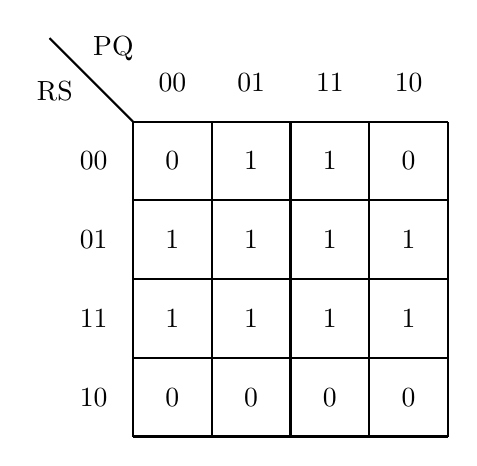
\begin{tikzpicture}
\draw (0,0) grid (4,4);
  \draw (0,4) -- node [pos=0.6,above right,anchor=south west] {PQ} node [pos=0.6,below left,anchor=north east]
        {RS} ++(135:1.5);
  % Draw vertical lines
  \foreach \x in {0,1,2,3,4}
    \draw (\x,0) -- (\x,4);
  % Draw horizontal lines
  \foreach \y in {0,1,2,3,4}
    \draw (0,\y) -- (4,\y);
  % Draw cell labels
  %4th row
  \node at (0.5,0.5) {0};
  \node at (1.5,0.5) {0};
  \node at (2.5,0.5) {0};
  \node at (3.5,0.5) {0};
  %3rd row
  \node at (0.5,1.5) {1};
  \node at (1.5,1.5) {1};
  \node at (2.5,1.5) {1};
  \node at (3.5,1.5) {1};
  %2nd row
  \node at (0.5,2.5) {1};
  \node at (1.5,2.5) {1};
  \node at (2.5,2.5) {1};
  \node at (3.5,2.5) {1};
  %1st row
  \node at (0.5,3.5) {0};
  \node at (1.5,3.5) {1};
  \node at (2.5,3.5) {1};
  \node at (3.5,3.5) {0};
  % Draw index labels
  \foreach \x/\val in {0/00,1/01,2/11,3/10}
    \node at (\x+0.5,4.5) {\val};
   % Draw index labels    
  \foreach \y/\val in {3/00,2/01,1/11,0/10}
    \node at (-0.5,\y+0.5) {\val};
\end{tikzpicture}
                        \caption{}
                        \label{fig:kmap}
\end{center}
\end{figure}
\begin{enumerate}
  \item QR'+S
  \item QR+S
    \item QR'+S'
    \item QR+S'
\end{enumerate}

\item In the circuit shown below , X and Y are digital inputs, and Z is a digital output. The quivalent 
		circuit is a  
		\label{prob:2019 EE 36}
		\hfill(GATE EE 2019)
\begin{figure}[htbp]
\begin{center}
    \centering
    \begin{circuitikz}[scale=1]
    % 1st not
        \draw (0,0) node[not port,scale=0.8 ] (not) {};
        \draw (3,-0.28) node[and port] (and) {};
        
        \draw (not.in 1) -- ++(-1,0) node[left] {$X$};
        \draw (not.out) -- ++(0,0) coordinate (and.in 1);
        \draw (not.in 1) -- ++(0,-1.7) node[below] {$ $};
    % 1st And
        \draw (and.in 1) -- ++(-1.2,0) node[left] {$ $};
        \draw (and.in 2) -- ++(-3.3,0) node[left] {$Y$};
        \draw (and.out) -- ++(0,0) node[right] {$ $};

        \draw (and.in 2) -- ++(-3,0) coordinate (point);
        \draw (point) -- ++(0,-1.7) -- ++(1,0) node[below] {$ $};
        \draw (and.out) -- ++(0,-0.47) node[below] {$ $};
    %2nd not
        \draw (0,-2.28) node[not port ,scale=0.8] (not) {};
        \draw (not.in 1) -- ++(-0.8,0) node[left] {$ $};
        \draw (not.out) -- ++(0,0) coordinate (and.in 2);
   %2nd ANd
        \draw (3,-2) node[and port] (and) {};
        \draw (and.in 1) -- ++(-2.2,0) node[left] {$ $} ;
        \draw (and.in 2) -- ++(-1.2,0) node[left] {$ $} ;
        \draw (and.out) -- ++(0,0) node[right] {$ $};
          \draw (and.out) -- ++(0,0.7) node[above] {$ $};
    %or
        \draw (6,-1) node[or port] (or) {};
        \draw (or.in 1) -- ++(-1.48,0) node[left] {$ $} ;
        \draw (or.in 2) -- ++(-1.48,0) node[left] {$ $} ;
        \draw (or.out) -- ++(1,0) node[right] {$Z$};
     \end{circuitikz}
	\caption{ }
	\label{fig}
\end{center}
\end{figure}
    \begin{enumerate}
        \item NAND gate
        \item NOR gate
        \item XOR gate
        \item XNOR gate
    \end{enumerate}
    \item 
	\label{prob:gate IN 23}
	The output F of the digital circuit shown can be written in the form(s)\rule{2cm}{0.4pt}
	\hfill(GATE IN 2022)
	\begin{figure}[H]
	\begin{circuitikz}[x=0.75pt,y=0.75pt,yscale=-1,xscale=1] 
%uncomment if require: \path (0,300); %set diagram left start at 0, and has height of 300 
 
%Shape: Rectangle [id:dp6333282224419394]  
\draw   (152,97) -- (232,97) -- (232,204) -- (152,204) -- cycle ; 
%Shape: Rectangle [id:dp18165331400027773]  
\draw   (308,97) -- (388,97) -- (388,203) -- (308,203) -- cycle ; 
%Straight Lines [id:da19243851950817237]  
\draw    (105,123) -- (151,123) ; 
%Straight Lines [id:da5189250982732854]  
\draw    (107,166) -- (152,167) ; 
%Straight Lines [id:da10677894123694709]  
\draw    (233,145) -- (271,145) -- (271,178) -- (310,178) ; 
%Straight Lines [id:da945249451843431]  
\draw    (271,122) -- (308,122) ; 
%Straight Lines [id:da4925880084299934]  
\draw    (194,204) -- (194,237) ; 
%Straight Lines [id:da06719238704994501]  
\draw    (349,202) -- (350,237) ; 
%Straight Lines [id:da6955179199661197]  
\draw    (389,148) -- (431,150) ;  
% Text Node 
\draw (171,130) node [anchor=north west][inner sep=0.75pt]   [align=left] {2x1\\MUX}; 
% Text Node 
\draw (331,130) node [anchor=north west][inner sep=0.75pt]   [align=left] {2x1\\MUX}; 
% Text Node 
\draw (103,99) node [anchor=north west][inner sep=0.75pt]   [align=left] {1}; 
% Text Node 
\draw (106,144) node [anchor=north west][inner sep=0.75pt]   [align=left] {0}; 
% Text Node 
\draw (155,116) node [anchor=north west][inner sep=0.75pt]  [font=\scriptsize] [align=left] {$I_0$}; 
% Text Node 
\draw (312,113) node [anchor=north west][inner sep=0.75pt]  [font=\scriptsize] [align=left] {$I_0$}; 
% Text Node 
\draw (312,170) node [anchor=north west][inner sep=0.75pt]  [font=\scriptsize] [align=left] {$I_1$}; 
% Text Node 
\draw (156,160) node [anchor=north west][inner sep=0.75pt]  [font=\scriptsize] [align=left] {$I_1$}; 
% Text Node 
\draw (357,224) node [anchor=north west][inner sep=0.75pt]   [align=left] {A}; 
% Text Node 
\draw (201,224) node [anchor=north west][inner sep=0.75pt]   [align=left] {B}; 
% Text Node 
\draw (425,130) node [anchor=north west][inner sep=0.75pt]   [align=left] {F}; 
% Text Node 
\draw (185,187) node [anchor=north west][inner sep=0.75pt]  [font=\scriptsize] [align=left] {$S_0$}; 
% Text Node 
\draw (341,186) node [anchor=north west][inner sep=0.75pt]  [font=\scriptsize] [align=left] {$S_0$}; 
\end{circuitikz}
		\caption{}
		\label{figure}
	\end{figure}
		\begin{enumerate}
       			\item $\overline {A \cdot B}$
    			\item $\overline A$+$\overline B$
     			\item $\overline{A+B}$
 			\item $\overline A \cdot \overline B$			
		\end{enumerate}
            \item 
            \label{prob:gate IN 35}
            If $X = X_1X_0$ and $Y = Y_1Y_0$ are 2-bit binary numbers. The Boolean function S that satisfies the condition "If $X \textgreater Y$, then $S= 1$", in its minimized form, is ?\\
                  \begin{enumerate}
 
                        \item$X_1Y_1$+$X_0Y_0$
                        \item$X_1\overline{Y_1}+X_0\overline{Y_0}\overline{Y_1}+X_0\overline{Y_0}X_1$
                        \item$X_1\overline{Y_1}X_0\overline{Y_0}$
                        \item$X_1Y_1+X_0\overline{Y_0}Y_1+X_0\overline{Y_0}\overline{X_1}$
                  \end{enumerate}
            \hfill(GATE IN 2019)
\item
\label{prob:gate IN 22}
     The figure below shows the $i^{th}$ full-adder block of a binary adder circuit.$C_{i}$  is the input carry and $C_{i+1}$ is the output carry of the circuit. Assume that each logic gate has a delay of $2$ nanosecond, with no additional time delay due to the interconnecting wires. Of the inputs $A_{i}$ , $B_{i}$ are available and stable throughout the carry propagation, the maximum time taken for an input $C_{i}$ to produce a steady-state output $C_{i+1}$ is $\underline{\hspace{2cm}}$ nanosecond.
     \hfill(GATE IN 2019)
     \begin{figure}[H]
     \begin{circuitikz}
    \draw (1.5, 1.5) node[xor port] (xor1) {};
    \draw (xor1.in 1) -- ++(-1.0,0) node[anchor=east] {$A_i$};
    \draw (xor1.in 2) -- ++(-1.0,0) node[anchor=east] {$B_i$};
    \draw (1.5, 1.5) -- (3.0, 1.5);
    \draw (-0.1, 1.3) -- (-0.1, -1.2);
    \draw (-0.5, 1.8 ) -- (-0.5, -1.8);
    \draw (-0.1, -1.2) -- (0.5, -1.2);
    \draw (-0.5, -1.8) -- (0.5, -1.8);
    \draw (1.8, -1.5) node[and port] (and 1) {};
    \draw (4.1, 1.2) node[xor port] (xor2)  {};
    \draw (2.8, 0.9) -- (2.8, -3.3);
    \draw (2.8, -3.3) -- (-1.0, -3.3);
    \draw (-1.0,-3.3) node[anchor=east] {$C_in$};
    \draw (2.0, 1.5) -- (2.0, -0.3);
    \draw (2.0, -0.3) -- (3.1, -0.3);
    \draw (4.2, -0.6) node[and port] (and 2) {};
    \draw (1.8, -1.5) -- (5.8, -1.5);
    \draw (4.2, -0.6) -- (6.0, -0.6);
    \draw (7.2, -0.9) node[xor port] (xor3) {};
    \draw (5.8, -1.5) -- (5.8, -1.2);
    \draw (4.8, 1.2) node[anchor = east] {$S_i$};
    \draw (8.7, -0.9) node[anchor=east] {$C_{i+1}$};
\end{circuitikz}
\caption{}
\label{figiure_kmap}
\end{figure}
\item
\label{prob:gate IN 43}
The Product of sun expression of a Boolean function
                $F(A,B,C)$ three variables is given by 
                \begin{align}
                   F(A,B,C)=(A+B+\overline{C})\times(A+\overline{B}+\overline{C}\times(\overline{A}+B+C)\times(\overline{A}+\overline{B}+\overline{C})
                \end{align}
                The canonical sum of product expression of $F(A,B,C)$ is given by 
                 \begin{enumerate}
 
            \item$\overline{A}\overline{B}C+\overline{A}BC+A\overline{B}\overline{C}+ABC$
            \item$\overline{ABC}+\overline{A}B\overline{C}+A\overline{B}C+AB\overline{C}$
            \item$A B\overline{C}+A\overline{B C}+\overline{A}B C+\overline{ABC}$
            \item$\overline{ABC}+\overline{A}BC+AB\overline{C}+ABC$
                  \end{enumerate}
		\hfill(GATE IN 2018)
\item
	\label{prob:gate EC 31}
	A four-variable Boolean function is realized using $4\times 1$ multiplexers as shown in the figure.
    \begin{figure}[!h]
        \centering
        \includegraphics[width=\columnwidth]{figs/2018-gate-ec-31.png}
        \caption{}
        \label{fig:mux}
    \end{figure}

   The minimized expression for 
    \begin{enumerate}
       \item $\left ( UV+\bar{U}\bar{V} \right )\bar{W}$
       \item $\left ( UV+\bar{U}\bar{V} \right )\left ( \bar{W}\bar{X}+\bar{W}X\right )$
       \item $\left ( U\bar{V}+\bar{U}V \right )\bar{W}$
       \item $\left ( U\bar{V}+\bar{U}V \right )\left ( \bar{W}\bar{X}+\bar{W}X\right )$

    \end{enumerate}
    \hfill(GATE EC 2018)

\item
	\label{prob:2023-gate-ec-9}
	A function $F(A, B, C)$ defined by three Boolean variables A, B and C when expressed as sum of products is given by \newline$ F = \brak{\overline{A} \cdot \overline{B} \cdot \overline{C}} + \brak{\overline{A} \cdot B \cdot \overline{C}} + \brak{A \cdot \overline{B} \cdot \overline{C}} $
where, $\overline{A},\overline{B}$ and $\overline{C}$ are the complements of the respective variables.The product of sums (POS) form of the function F is

\begin{enumerate}[label=(\Alph*)]
	\item $ \brak{A+B+C} \cdot \brak{A+\overline{B}+C} \cdot \brak{\overline{A}+B+C} $
 	\item $ \brak{\overline{A}+\overline{B}+\overline{C}} \cdot \brak{\overline{A}+B+\overline{C}} \cdot \brak{A+\overline{B}+\overline{C}} $
	\item $ \brak{A+B+\overline{C}} \cdot \brak{A+\overline{B}+\overline{C}} \cdot \brak{\overline{A}+B+\overline{C}} \cdot \brak{\overline{A}+\overline{B}+C} \cdot \brak{\overline{A}+\overline{B}+C} $
	\item $ \brak{\overline{A}+\overline{B}+C} \cdot \brak{\overline{A}+B+C} \cdot \brak{A+\overline{B}+C} \cdot \brak{A+B+\overline{C}} \cdot \brak{A+B+C} $
\end{enumerate}
\hfill(GATE EC 2018)




    \item 
        \label{prob:gate EC 9}
	 In the circiut shown below , assume that the comparators are ideal and all components have zero propagation delay . In one period of the input signal Vin=6sin(wt),the fraction of the time which the output OUT is in login state HIGH is 

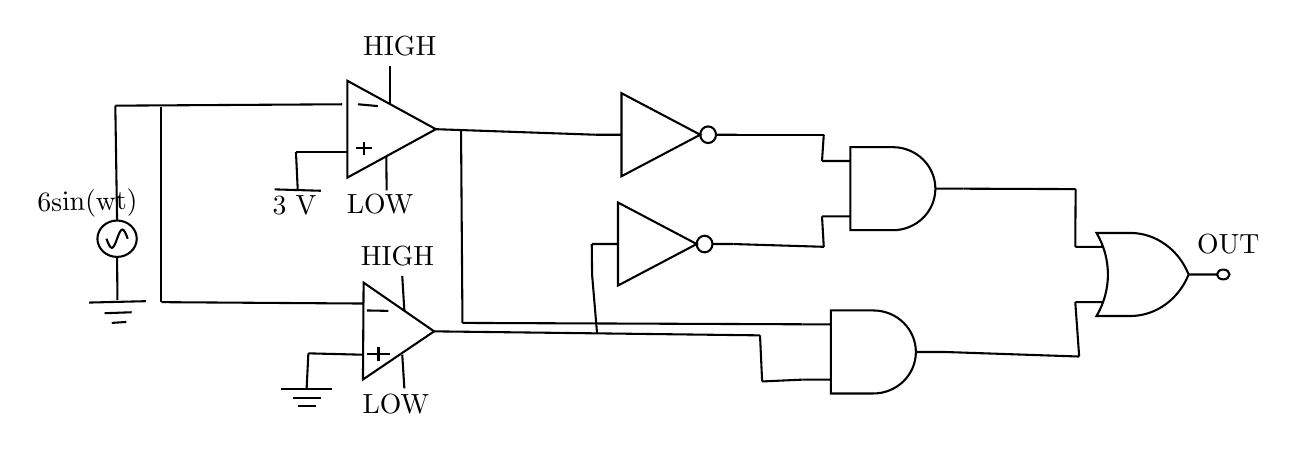
\begin{tikzpicture}[x=0.8pt,y=0.5pt,yscale=-1,xscale=0.8]
\tikzset{every picture/.style={line width=0.75pt}} %set default line width to 0.75pt        
%Straight Lines [id:da497014729381388] 
\draw    (140,132.6) -- (169,132.6) ;
%Flowchart: Extract [id:dp3321780746660581] 
\draw   (219,116) -- (169,151) -- (169,81) -- cycle ;
%Straight Lines [id:da17793857448296313] 
\draw    (38,99) -- (166,98) ;
%Straight Lines [id:da9757576729769633] 
\draw    (38,99) -- (39,182) ;
%Straight Lines [id:da772216831020951] 
\draw    (64,100) -- (64,241) ;
%Straight Lines [id:da17160688891184805] 
\draw    (140,132.6) -- (141,160) ;
%Flowchart: Extract [id:dp1753151070852037] 
\draw   (218,262.1) -- (177.82,296.89) -- (178.18,226.9) -- cycle ;
%Straight Lines [id:da8490718483620778] 
\draw    (64,241) -- (178,242) ;
%Straight Lines [id:da2131290241855488] 
\draw    (147,278) -- (146,304) ;
%Straight Lines [id:da06754998827437309] 
\draw    (147,278) -- (178,279) ;
%Straight Lines [id:da6585658480786443] 
\draw    (128,159.5) -- (154,160.5) ;
%Straight Lines [id:da38485782506888055] 
\draw    (131.5,304) -- (139.2,304) -- (160.5,304) ;
%Straight Lines [id:da9940160044670818] 
\draw    (219,116) -- (309,120) ;
%Shape: Not/Inverter Gate [id:dp6645899938254611] 
\draw   (323.81,90) -- (368.26,120) -- (323.81,150) -- (323.81,90) -- cycle (309,120) -- (323.81,120) (377.15,120) -- (389,120) (368.26,120) .. controls (368.26,116.69) and (370.25,114) .. (372.7,114) .. controls (375.16,114) and (377.15,116.69) .. (377.15,120) .. controls (377.15,123.31) and (375.16,126) .. (372.7,126) .. controls (370.25,126) and (368.26,123.31) .. (368.26,120) -- cycle ;
%Shape: Not/Inverter Gate [id:dp5203526386809565] 
\draw   (321.81,169) -- (366.26,199) -- (321.81,229) -- (321.81,169) -- cycle (307,199) -- (321.81,199) (375.15,199) -- (387,199) (366.26,199) .. controls (366.26,195.69) and (368.25,193) .. (370.7,193) .. controls (373.16,193) and (375.15,195.69) .. (375.15,199) .. controls (375.15,202.31) and (373.16,205) .. (370.7,205) .. controls (368.25,205) and (366.26,202.31) .. (366.26,199) -- cycle ;
%Shape: And Gate [id:dp9113043452641065] 
\draw   (453,129) -- (477,129) .. controls (490.25,129) and (501,142.44) .. (501,159) .. controls (501,175.56) and (490.25,189) .. (477,189) -- (453,189) -- (453,129) -- cycle (437,139) -- (453,139) (437,179) -- (453,179) (501,159) -- (517,159) ;
%Straight Lines [id:da5047558236731997] 
\draw    (389,120) -- (438,120) ;
%Straight Lines [id:da7853309017572672] 
\draw    (438,120) -- (437,139) ;
%Straight Lines [id:da09581339031746183] 
\draw    (437,179) -- (438,201) ;
%Straight Lines [id:da16150015131708795] 
\draw    (233.2,117.3) -- (234,256) ;
%Straight Lines [id:da3982360427353082] 
\draw    (218,262.1) -- (402,265) ;
%Straight Lines [id:da7763866390601679] 
\draw    (307.2,221.3) -- (310,263.55) ;
%Shape: And Gate [id:dp6929958094484654] 
\draw   (442,247) -- (466,247) .. controls (479.25,247) and (490,260.44) .. (490,277) .. controls (490,293.56) and (479.25,307) .. (466,307) -- (442,307) -- (442,247) -- cycle (426,257) -- (442,257) (426,297) -- (442,297) (490,277) -- (506,277) ;
%Straight Lines [id:da5339653129723407] 
\draw    (234,256) -- (426,257) ;
%Straight Lines [id:da3839391248130781] 
\draw    (307,199) -- (307.2,221.3) ;
%Straight Lines [id:da6726109915230507] 
\draw    (387,199) -- (438,201) ;
%Straight Lines [id:da40951430114554754] 
\draw    (402,265) -- (403.2,298.3) ;
%Straight Lines [id:da9775921532117686] 
\draw    (403.2,298.3) -- (426,297) ;
%Flowchart: Connector [id:dp8541564806415127] 
\draw   (27.9,195.15) .. controls (27.9,187.89) and (32.87,182) .. (39,182) .. controls (45.13,182) and (50.1,187.89) .. (50.1,195.15) .. controls (50.1,202.41) and (45.13,208.3) .. (39,208.3) .. controls (32.87,208.3) and (27.9,202.41) .. (27.9,195.15) -- cycle ;
%Shape: Sine Wave Form [id:dp42157572682524824] 
\draw   (33,195.15) .. controls (35.44,203.92) and (36.59,203.96) .. (39,195.15) .. controls (41.41,186.34) and (42.54,186.28) .. (45,195.15) ;
%Shape: Or Gate [id:dp7839680372805569] 
\draw   (592,191) -- (612,191) .. controls (625.95,191.54) and (638.42,203.23) .. (644,221) .. controls (638.42,238.77) and (625.95,250.46) .. (612,251) -- (592,251) .. controls (600.57,232.44) and (600.57,209.56) .. (592,191) -- cycle (580,201) -- (596,201) (580,241) -- (596,241) (644,221) -- (660,221) ;
%Straight Lines [id:da1579523714650295] 
\draw    (517,159) -- (580.2,159.3) ;
%Straight Lines [id:da6248594806976522] 
\draw    (506,277) -- (582.2,280.3) ;
%Straight Lines [id:da07782234715989711] 
\draw    (580.2,159.3) -- (580,201) ;
%Straight Lines [id:da20731054042333286] 
\draw    (580,241) -- (582.2,280.3) ;
%Straight Lines [id:da4591115076560359] 
\draw    (193.2,70.3) -- (193.2,98.3) ;
%Straight Lines [id:da9614915073120633] 
\draw    (191,136) -- (191.2,160.3) ;
%Straight Lines [id:da6267154334794827] 
\draw    (200,279) -- (201.2,303.3) ;
%Straight Lines [id:da7013095252421617] 
\draw    (200,222) -- (201.2,247.3) ;
%Straight Lines [id:da505762670676958] 
\draw    (141.2,316.3) -- (151.2,316.3) ;
%Straight Lines [id:da5523950339641612] 
\draw    (175,98) -- (186.2,99.3) ;
%Straight Lines [id:da3727188903283414] 
\draw    (138.2,310.3) -- (154.2,310.3) ;
\draw   (174,129.65) -- (183.2,129.65)(178.6,125) -- (178.6,134.3) ;
\draw   (180,278.3) -- (193.2,278.3)(186.6,273.3) -- (186.6,283.3) ;
%Straight Lines [id:da6667775045429274] 
\draw    (180,247) -- (192.2,247.3) ;
%Shape: Circle [id:dp7754800448867729] 
\draw   (660,221) .. controls (660,219.04) and (661.59,217.45) .. (663.55,217.45) .. controls (665.51,217.45) and (667.1,219.04) .. (667.1,221) .. controls (667.1,222.96) and (665.51,224.55) .. (663.55,224.55) .. controls (661.59,224.55) and (660,222.96) .. (660,221) -- cycle ;
%Straight Lines [id:da3040090400300808] 
\draw    (39,208.3) -- (39.2,239.6) ;
%Straight Lines [id:da6746368970911716] 
\draw    (23.2,241.3) -- (55.2,240.3) ;
%Straight Lines [id:da7013568848674232] 
\draw    (32,249) -- (47.2,248.3) ;
%Straight Lines [id:da40668201779662905] 
\draw    (36,256) -- (44.2,255.3) ;

% Text Node
\draw (199.7,56.16) node  [rotate=-359.96] [align=left] {\begin{minipage}[lt]{27.88pt}\setlength\topsep{0pt}
HIGH
\end{minipage}};
% Text Node
\draw (190.6,170.15) node   [align=left] {\begin{minipage}[lt]{28.02pt}\setlength\topsep{0pt}
LOW
\end{minipage}};
% Text Node
\draw (201.78,207.75) node   [align=left] {\begin{minipage}[lt]{32.1pt}\setlength\topsep{0pt}
HIGH
\end{minipage}};
% Text Node
\draw (200.1,314.75) node   [align=left] {\begin{minipage}[lt]{28.7pt}\setlength\topsep{0pt}
LOW
\end{minipage}};
% Text Node
\draw (669.1,198.75) node   [align=left] {\begin{minipage}[lt]{25.98pt}\setlength\topsep{0pt}
OUT
\end{minipage}};
% Text Node
\draw (12.13,170) node  [rotate=-358.82] [align=left] {\begin{minipage}[lt]{23.22pt}\setlength\topsep{0pt}
6sin(wt)
\end{minipage}};
% Text Node
\draw (146.6,170.65) node   [align=left] {\begin{minipage}[lt]{25.3pt}\setlength\topsep{0pt}
3 V
\end{minipage}};
\end{tikzpicture}
\begin{enumerate}
    \item $\frac{1}{12}$
    \item $\frac{1}{2}$
    \item $\frac{2}{3}$
    \item $\frac{5}{6}$
\end{enumerate}
\hfill(GATE EC 2018)




  \item 
  \label{prob:gate  IN 46}
  The Boolean function $F\brak{X,Y}$ realized by the given circuit is
  
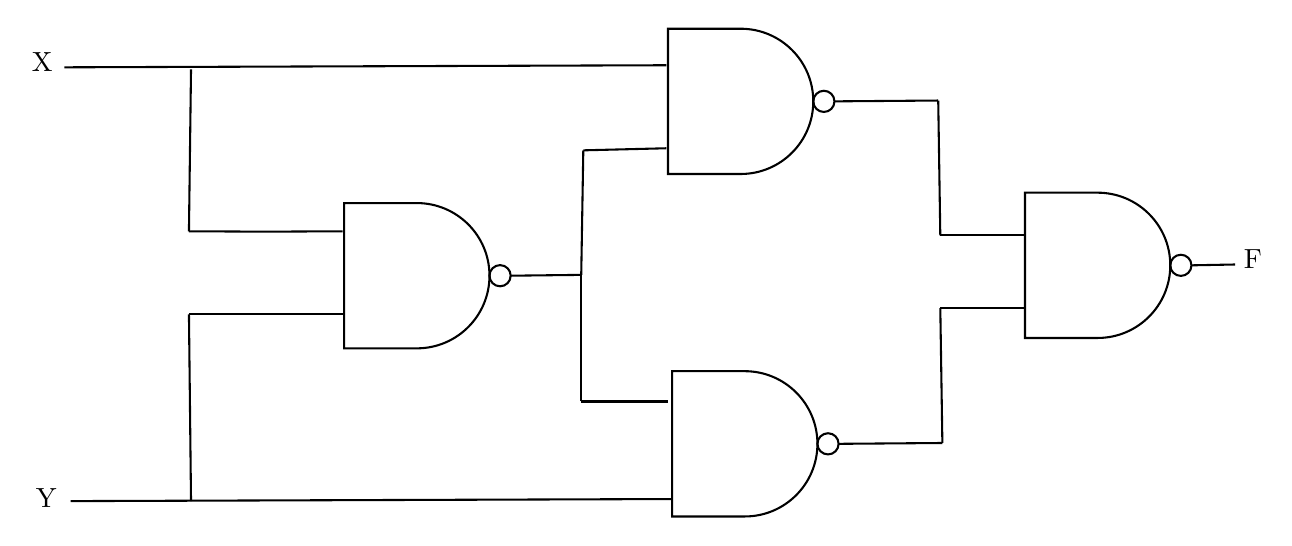
\begin{tikzpicture}[x=0.75pt,y=0.75pt,yscale=-1,xscale=1]
% Your original TikZ code here
\tikzset{every picture/.style={line width=0.75pt}} %set default line width to 0.75pt        

%Straight Lines [id:da8870235423908663] 
\draw    (99.2,109.6) -- (136.21,109.78) -- (173.2,109.6) ;
%Flowchart: Delay [id:dp3076178503272544] 
\draw   (174,96) -- (209,96) .. controls (228.33,96) and (244,111.67) .. (244,131) .. controls (244,150.33) and (228.33,166) .. (209,166) -- (174,166) -- cycle ;
%Straight Lines [id:da4880418888531195] 
\draw    (99.2,149.6) -- (111.2,149.6) -- (166.2,149.6) -- (174.2,149.6) ;
%Shape: Circle [id:dp4693486828792446] 
\draw   (244,131) .. controls (244,128.18) and (246.28,125.9) .. (249.1,125.9) .. controls (251.92,125.9) and (254.2,128.18) .. (254.2,131) .. controls (254.2,133.82) and (251.92,136.1) .. (249.1,136.1) .. controls (246.28,136.1) and (244,133.82) .. (244,131) -- cycle ;
%Straight Lines [id:da4653941185722381] 
\draw    (254.2,131) -- (288.2,130.6) ;
%Straight Lines [id:da8761511817778416] 
\draw    (39.2,30.6) -- (329.2,29.6) ;
%Straight Lines [id:da1606414736134072] 
\draw    (42.2,239.6) -- (332.2,238.6) ;
%Straight Lines [id:da6304107801712311] 
\draw    (288.2,130.6) -- (289.2,70.6) ;
%Straight Lines [id:da9368244337166334] 
\draw    (289.2,70.6) -- (329.2,69.6) ;
%Straight Lines [id:da8466357262704003] 
\draw    (288.2,191.6) -- (288.2,130.6) ;
%Straight Lines [id:da46784195426353525] 
\draw    (288.2,191.6) -- (330.2,191.6) ;
%Flowchart: Delay [id:dp9030516796824679] 
\draw   (330,12) -- (365,12) .. controls (384.33,12) and (400,27.67) .. (400,47) .. controls (400,66.33) and (384.33,82) .. (365,82) -- (330,82) -- cycle ;
%Flowchart: Delay [id:dp09252224992976132] 
\draw   (332,177) -- (367,177) .. controls (386.33,177) and (402,192.67) .. (402,212) .. controls (402,231.33) and (386.33,247) .. (367,247) -- (332,247) -- cycle ;
%Shape: Circle [id:dp5499693136350294] 
\draw   (402,212) .. controls (402,209.18) and (404.28,206.9) .. (407.1,206.9) .. controls (409.92,206.9) and (412.2,209.18) .. (412.2,212) .. controls (412.2,214.82) and (409.92,217.1) .. (407.1,217.1) .. controls (404.28,217.1) and (402,214.82) .. (402,212) -- cycle ;
%Shape: Circle [id:dp74153314191801] 
\draw   (400,47) .. controls (400,44.18) and (402.28,41.9) .. (405.1,41.9) .. controls (407.92,41.9) and (410.2,44.18) .. (410.2,47) .. controls (410.2,49.82) and (407.92,52.1) .. (405.1,52.1) .. controls (402.28,52.1) and (400,49.82) .. (400,47) -- cycle ;
%Straight Lines [id:da35345529297391987] 
\draw    (410.2,47) -- (460.2,46.6) ;
%Straight Lines [id:da8140464066015929] 
\draw    (412.2,212) -- (462.2,211.6) ;
%Flowchart: Delay [id:dp21989758956535077] 
\draw   (502,91) -- (537,91) .. controls (556.33,91) and (572,106.67) .. (572,126) .. controls (572,145.33) and (556.33,161) .. (537,161) -- (502,161) -- cycle ;
%Straight Lines [id:da14664335527509076] 
\draw    (460.2,46.6) -- (461.2,111.6) ;
%Straight Lines [id:da5388257463322341] 
\draw    (461.2,146.6) -- (462.2,211.6) ;
%Straight Lines [id:da4857250526271579] 
\draw    (461.2,111.6) -- (502.2,111.6) ;
%Straight Lines [id:da5555292815908546] 
\draw    (461.2,146.6) -- (502.2,146.6) ;
%Shape: Circle [id:dp793166461459196] 
\draw   (572,126) .. controls (572,123.18) and (574.28,120.9) .. (577.1,120.9) .. controls (579.92,120.9) and (582.2,123.18) .. (582.2,126) .. controls (582.2,128.82) and (579.92,131.1) .. (577.1,131.1) .. controls (574.28,131.1) and (572,128.82) .. (572,126) -- cycle ;
%Straight Lines [id:da6138015275286377] 
\draw    (582.2,126) -- (603.2,125.6) ;
%Straight Lines [id:da6694995059558879] 
\draw    (99.2,109.6) -- (100.2,31.6) ;
%Straight Lines [id:da9757039240740732] 
\draw    (100.2,239.6) -- (99.2,149.6) ;

% Text Node
\draw (22,22) node [anchor=north west][inner sep=0.75pt]   [align=left] {X};
% Text Node
\draw (24,232) node [anchor=north west][inner sep=0.75pt]   [align=left] {Y};
% Text Node
\draw (606,117) node [anchor=north west][inner sep=0.75pt]   [align=left] {F};

  
\end{tikzpicture}
\begin{enumerate}
      \item \(\bar{X}Y + X\bar{Y}\)
      \item \(\bar{X}\bar{Y} + XY\)
      \item \(X+Y\)
      \item \(\bar{X}.\bar{Y}\)

      \end{enumerate}
\hfill(GATE IN 2019)


  \item 
  \label{prob:gate  CS 49 }
 Consider the minterm list form of a Boolean function given below.\\$F(P, Q, R, S) = \sum m(0, 2, 5, 7, 9, 11) + d(3, 8, 10, 12, 14)$\\
Here, denotes a minterm and denotes a don’t care term. The number of essential prime implicants of the function is
\hfill(GATE CS 2018)
\end{enumerate}
